%!TeX TXS-program:clean = latexmk.exe -c %
%!TeX TXS-program:quick = txs:///compile | txs:///biber | txs:///compile | txs:///view | txs:///clean
%!TeX TXS-program:bibliography = txs:///biber
%!BIB program = biber
\documentclass[12pt,letterpaper]{article}

% Essential Math and Symbol Packages
\usepackage{amsmath,amssymb,amsthm}
\usepackage{mathtools}
\usepackage{geometry}
\usepackage[style=apa,backend=biber]{biblatex}
\geometry{margin=1in}
\setlength{\parindent}{0pt}
\addbibresource{references.bib}

% Theorem Environments Setup
\newtheorem{theorem}{Theorem}[section]
\newtheorem{lemma}[theorem]{Lemma}
\newtheorem{definition}[theorem]{Definition}
\newtheorem{proposition}[theorem]{Proposition}
\newtheorem{corollary}[theorem]{Corollary}

\title{A Cortico-Cerebellar model}
\author{Luis Luarte}
\date{\today}

\begin{document}
	\maketitle
	
	\begin{abstract}
		a
	\end{abstract}
	
	\section{Introduction}
	The Marr-Albus-Ito framework modeled the cerebellum as a feedforward error-corrector \parencite{marrTheoryCerebellarCortex1969, albusTheoryCerebellarFunction1971, itoControlMentalActivities2008}. Further work on cerebellum models included paired forward and inverse controllers, which represent computational modules where the forward model predicts future sensory states from current motor commands, and the inverse model computes the necessary commands to achieve a desired target state \parencite{harunoMosaicModelSensorimotor2001, mehtaForwardModelsVisuomotor2002}. More recently cerebellum models have added large-scale spiking networks, that is, biologically constrained simulations tracking discrete membrane voltage integrations and action potentials across cerebellar layers \parencite{hoangPredictiveRewardpredictionErrors2025, verduzco-floresHowCreditAssignment2015}. These architectures integrate cortico-cerebellar connectivity, demonstrating that climbing fibers encode reward-prediction errors (RPEs) rather than purely motor execution related errors \parencite{hoangPredictiveRewardpredictionErrors2025, jinRewarddrivenCerebellarClimbing2024}. This implies relevant cerebellar involvement in cognitive processing \parencite{schmahmannDysmetriaThoughtClinical1998a} and reward processing \parencite{hullPredictionSignalsCerebellum2020}. 
	
	While these models incorporate the cerebellum into reinforcement learning, frequently using localized eligibility traces at the parallel fuber-Purkinje synapse to resolve delayed credit assignment \parencite{verduzco-floresHowCreditAssignment2015, doyaWhatAreComputations1999}, they utilze these temporal buffer strictly to compute terminal action values or motor commands, omitting the dynamical loop that connects the cerebellar computation back to the cortical manifold. Where the cortical manifold is the representation of the space where cognitive trajectories are computed or processed over time. This structural omission (positioning the cerebellum as a strict in-parallel unit) has been formally recognized as a severe constraint in recent consensus papers demanding unified predictive loops \parencite{kakeiConsensusPaperModels2026, miallStateEstimationCerebellum2008}. Thus while the cerebellum may internally bridge information to the cortex, this constrains models to Markovian environments (tasks where the instantaneous sensory observation contains all necessary information for optimal action selection, mathematically rendering historical states redundant).
	
	The constraint to Markovian regimes is a persistent structural constant across the chronology of computational cerebellar modeling. This can be derived from three cannonical cerebellum computational models.
	\begin{enumerate}
		\item \textbf{Adaptive Filter Models \parencite{fujitaAdaptiveFilterModel1982}:} These models define the cerebellar output $y_t$ as a linear combination of parallel fiber inputs $x_i$, where each input is delayed by a distinct temporal offset $\tau_i$ (representing tapped delay lines) and multiplied by a modifiable synaptic weight $w_i$, yielding $y_t = \sum_i w_i x_i(t-\tau_i)$. While this design maps temporally disparate inputs to resolve an immediate motor error, the architecture is purely feedforward. In dynamical systems, the Jacobian matrix contains the first-order partial derivatives that define how a change in one vector perturbs the future trajectory of another. Here, the Jacobian mapping the cerebellar output back to the future cortical state is identically null ($\frac{\partial x_{t+1}}{\partial y_t} = 0$). Because the cerebellar output exerts zero recurrent mathematical influence on the subsequent cortical state $x_{t+1}$, the temporal history ($t-\tau_i$) processed by the cerebellum is never returned to the cortex. Consequently, the cortex cannot access past latencies; it is forced to compute its next state solely using its instantaneous observation, thus performing only in a Markovian setting.
		
		\item \textbf{Modular Internal Models (MOSAIC) \parencite{harunoMosaicModelSensorimotor2001}:} MOSAIC distributes learning across parallel modules governed by a responsibility signal $\lambda_t^{(i)} \propto \exp(-\|x_t - \hat{x}_{t}^{(i)}\|^2)$. In this formulation, $x_t$ is the actual sensory observation at time $t$, $\hat{x}_{t}^{(i)}$ is the sensory prediction generated by the $i$-th forward model, and the exponential function scales this instantaneous prediction error into a probability, activating the module whose current prediction is most accurate. Because this posterior responsibility is evaluated instantaneously against the current observation, the architecture requires that the immediate context vector completely resolves all state ambiguity. It lacks a continuous differential equation capable of propagating a unified trace over non-Markovian delays. A non-Markovian delay is a temporal gap between an action and its consequent feedback (the delay phase in trace conditioning or spatial working memory) where the current state is insufficient to link them. During this temporal gap, meaningful sensory errors evaluating the past action are temporarily absent from the environment. Because MOSAIC relies exclusively on instantaneous prediction errors to switch modules, it cannot bridge this void to assign credit to a historical state once the delayed feedback eventually arrives.
		
		\item \textbf{Cerebellar Reservoir Computing \parencite{yamazakiCerebellumLiquidState2007}:} Reservoir computing based models focus mainly on the Granule $\rightarrow$ Golgi network as a generator of robust temporal bases to build an information reservoir that can be read to decode information related to task state and value. A temporal basis is a sequence of time-varying, linearly independent spatial patterns of neural activity that encodes the time following a stimulus. By performing a time-to-space transformation, the network maps the scalar dimension of elapsed time into a continuous trajectory of unique, high-dimensional population states. This enables downstream readout neurons to decode arbitrary temporal delays through static spatial filtering, firing only when the specific population vector corresponding to a target delay emerges. This is mathematically defined by the recurrent state update $\mathbf{z}_t = f(\mathbf{W}_{\mathrm{rec}} \mathbf{z}_{t-1} + \mathbf{W}_{\mathrm{in}} \mathbf{x}_t)$, where $\mathbf{W}_{\mathrm{in}}$ is the input weight matrix mapping the external cortical signal (via mossy fibers) into the network, and $\mathbf{W}_{\mathrm{rec}}$ is the recurrent weight matrix defining the internal Granule-Golgi feedback dynamics that generate the fading temporal memory. However, the readout is an open-loop projection $y_t = \mathbf{W}_{\mathrm{out}} \mathbf{z}_t$. Because the reservoir state $\mathbf{z}_t$ never recursively perturbs the cortical driver $\mathbf{x}_t$, the temporal memory remains isolated in the cerebellum and cannot iterate the cortical representation itself.
	\end{enumerate}
	
	Evidently animals solve non-Markovian tasks in natural environments, capacity that seems to be deeply linked with the cortico-cerebellar loops that has received less attention in computational models. There is consistent evidence of a computational dissociation of the role of the Cerebellum in Markovian and non-Markovian tasks. Partial ablation of the Cerebellum spares Markovian performance while diminishing non-Markovian capabilities. In classical conditioning, \textcite{tsengSensoryPredictionErrors2007} shows that cerebellar lesions spare delay eyeblink conditioning (where the cue and reward overlap in time, $\tau = 0$); however, trace conditioning is absent (where a temporal gap requires bridging, $\tau > 0$). In human functional neuroimaging \parencite{habasDistinctCerebellarContributions2009, bucknerOrganizationHumanCerebellum2011}, the dentate nucleus does not produce a clear metabolic signal during simple, static motor execution, but becomes functionally coupled to the prefrontal cortex specifically during non-Markovian executive working memory tasks. These conditions, typically assessed via the $N$-back task or delayed-response paradigms, mandate that the subject actively maintain and continuously update a hidden sequence of cognitive states across multi-second temporal delays in the strict absence of immediate sensory cues. Causal experiment confirm this trend, optogenetically silenced cerebellar projection to the ventromedial thalamus, maintained simple cue-guided sensory mapping, while performance on delayed-response tasks requiring state maintenance was diminished \parencite{gaoCorticocerebellarLoopMotor2018}. Similarly, inactivation of cerebellar output node, maintain static assosiative learning, but diminish reversal, which require evaluation of historical actiona trajectories to update policies \parencite{chabrolCerebellarContributionPreparatory2019}. Finally, bilateral lesions of the ventral dentate nuclei in non-human primates, showed preservation of static recognition memory (delayed non-matching to sample) and basic motor execution, while abolishing spatial working memory (delayed recognition span task) and inducing perseveration in executive set-shifting (conceptual set shifting task).
	
	To solve this gap, we formalize a unified cortico-cerebellar framework that binds predictive coding, reservoir computing, and information geometry. Predictive coding is an inference framework where neural circuits continuously minimize the mismatch between top-down expectations and bottom-up sensory inputs \parencite{fristonPredictiveCodingFreeenergy2009}; we use its principles in our formulation as it provides a way to generate continuous sensory prediction errors ($\boldsymbol{\epsilon}_t$) that drive state-value updates in one go, without the need for non-biologically-plausible mechanisms such as back-propagation-through-time (BPTT). Reservoir computing utilizes fixed, recurrent networks of nonlinear nodes to project inputs into high-dimensional dynamic spaces \parencite{maassLiquidStateMachine2002, hauserTheoreticalFoundationMorphological2011}; we use it as the mathematical formalization of the Marr-Albus-Ito framework. This mathematically captures how the $\text{Mossy Fiber} \rightarrow \text{Granule Layer} \rightarrow \text{Golgi Cells}$ network generates a fading memory, a dynamical property where the influence of a past input on the current state decays over time, allowing the network to function as a finite historical buffer. This fading memory intrinsically enforces the linear separation of context by embedding similar inputs with divergent temporal histories into unique, non-overlapping high-dimensional population vectors, the reservoir renders ambiguous states linearly separable. This high-dimensional contextual separation is mathematically required to bridge non-Markovian structures, allowing the system to resolve temporally delayed credit assignment through simple spatial readouts. Information geometry analyzes neural state spaces as Riemannian manifolds, that is, continuous topological spaces equipped with a smoothly varying metric that defines the distances, angles, and separability between distinct neural population states, where distance metrics govern representational limits \parencite{amariNaturalGradientWorks1998}. This framework bounds our cortico-cerebellar projections by applying the Johnson-Lindenstrauss lemma to derive the strict minimum dimensionality required for the Deep Cerebellar Nuclei bottleneck, which compresses the expanded cerebellar state into a computationally feasible vector ($\mathbf{D}_t$) for transmission via the thalamus. Establishing this lower bound is critical to ensure that the recurrent loops preserve topological distances, maintaining the exact pairwise geometric distances between state vectors guarantees that the linear separability of historical contexts, achieved in the high-dimensional granule reservoir, is properly transmitted back to the cortical manifold. This metric preservation prevents the spatial representation from geometric failure where a rank-deficient or over-compressed projection forces distinct, non-Markovian temporal trajectories to map onto identical coordinates (a many-to-one mapping), destroying the contextual information required for delayed credit assignment.
	
	Here, we introduce a parameter-free distillation pipeline that compresses the unconstrained dynamics of an Oracle RNN into a biologically constrained, continuous-time cortico-cerebellar network via multi-objective Pareto optimization. To rigorously evaluate this architecture against empirical human data, we developed a custom adaptive Markov Chain Monte Carlo (MCMC) sampler. Using this custom Bayesian framework, we demonstrate that the continuous dynamical model quantitatively outperforms standard heuristic decision models in out-of-sample cross-validation. Furthermore, generative simulations of the fitted networks reveal emergent autonomous attractor dynamics; notably, the system sustains complex internal states during sensory deprivation that strictly depend on the integrity of the thalamic feedback loop.
	
	\section{Results}
		a
	
	\section{Methods}
	\subsection{Model specification}
	The model is divided into two main parts: (1) the Cortex, which acts as a generalized state-value learning algorithm and propogates the prediction error to (2) the Cerebellum, where via a expansion-sparsity-compression triad modifies a state representation that is used by the Cortex to generate further predictions.
	
	The cortical manifold operates under Predictive Coding, where sensory prediction errors ($\boldsymbol{\epsilon}_t$) drive a local Markovian gradient descent on the latent state ($\boldsymbol{\mu}_t$). To escape the Markovian limitation, the state is projected via Random Projections. By scattering the low-dimensional cortical state into a vastly higher dimension, random projections decorrelate spatially overlapping inputs, ensuring that states exhibiting instantaneous Markovian ambiguity become uniquely separable once embedded in the temporal dynamics of the reservoir. For this expansion, we use sparse Achlioptas matrices \parencite{achlioptasDatabasefriendlyRandomProjections2003} ($\mathbf{W}_{\mathrm{ach1}}$). These matrices are highly relevant as they mathematically guarantee metric preservation despite extreme sparsity (e.g., 90\% zero weights), accurately mirroring the biological sparsity of the mossy fiber-granule cell pathway to separate the low-dimensional cortical state into a high-dimensional linearly separable geometry (the Granule layer). Inside this layer, Reservoir Computing principles dictate the network dynamics, providing the physical fading memory necessary to buffer states across time. Within this expanded reservoir, Reinforcement Learning \parencite{suttonReinforcementLearningIntroduction2018} provides the temporal bridge: a physical eligibility trace ($\mathbf{Z}_t$) decays forward in time, capturing the delayed climbing fiber error via localized anti-Hebbian plasticity \parencite{itoCerebellarLongtermDepression2001}---a biological mechanism where parallel fiber synapses physically weaken when their recent activation coincides with a subsequent error signal ($\Delta \mathbf{W} \propto |\bar{\epsilon}_t| \mathbf{Z}_t$). 
	
	Finally, the system utilizes geometric \textbf{Compression and Sparsity}. Geometric compression forces a high-dimensional space into a lower-dimensional bottleneck while strictly preserving the pairwise topological distances between states, while sparsity minimizes energetic transmission costs by utilizing only a fraction of active nodes. A second Achlioptas projection bounds the network, preventing metric distortion as the updated historical trace is compressed back into the Deep Cerebellar Nuclei and continuously injected into the cortical manifold via the thalamus ($\beta_{\mathrm{thal}} \mathbf{D}_t$). Solving this connectivity transforms the cortex from an instantaneous sensory filter into an iterative, non-Markovian sequence generator. By recursively injecting the decaying cerebellar trace ($\mathbf{Z}_t$) back into the primary cortical state update, the network externalizes the temporal credit assignment problem, allowing the cortex to navigate delayed environments without maintaining an explicit memory of the past.
	
	\begin{equation}
		\hat{\mathbf{I}} = \mathbf{W}_{gen} \cdot \boldsymbol{\mu}_{t}\label{ctx_hallucination}
	\end{equation}
	
	\begin{equation}
		\epsilon = \Pi \odot (\mathbf{I}_{t} - \hat{\mathbf{I}}_{t})\label{ctx_pe}
	\end{equation}
	
	\begin{equation}
		\mathbf{G}_{t} = \mathbf{W}_{ach1} \cdot \boldsymbol{\mu}_{t}\label{gran}
	\end{equation}
	
	\begin{equation}
		\mathbf{Z}_{t} = (1 - \beta_{gran}) \cdot \mathbf{Z}_{t-1} + \alpha_{gran} \cdot \mathbf{G}_{t}\label{et}
	\end{equation}
	
	\begin{equation}
		\left| \bar{\epsilon} \right| = \frac{1}{d} \sum_{i=1}^{d} \left| \bar{\epsilon}_{t, i} \right|\label{c_pe}
	\end{equation}
	
	\begin{equation}
		\mathbf{W}_{purk, t} = \mathbf{W}_{purk, t-1} - \kappa ( \left| \bar{\epsilon} \right| \cdot \mathbf{Z}_{t})\label{purk}
	\end{equation}
	
	\begin{equation}
		\mathbf{D}_{t} = \mathbf{W}_{ach2} (\mathbf{G}_{t} \odot \mathbf{W}_{purk, t})\label{forward_pass}
	\end{equation}
	
	\begin{equation}
		\boldsymbol{\mu}_{t+1} = \boldsymbol{\mu}_{t} + \alpha_{c} [(\mathbf{W}^{T}_{gen} \cdot \epsilon_{t}) - (\lambda_{c} \cdot ITI_{t} \cdot \boldsymbol{\mu}_{t}) + \beta_{thal} (\mathbf{W}_{thal} \cdot \mathbf{D}_{t})]\label{thalam_ctx_pass}
	\end{equation}
	
	% linear readout equations
	\begin{equation}
		content...
	\end{equation}

	\subsection{Model parameter fit}
	
	\subsubsection{NSGA-II parameter discovery}
	
	We fitted an RNN to a sub-set of held-out data to generate the $RNN_{oracle}$ (see fig.\ref{fig:rnn_teacher_lnso})
	
	Then we extracted the $RNN_{oracle}$ predictions to provide a smoother optimization landscape to $Model_{student}$
	
	\subsubsection{Teacher-Student distillation}
	
	\subsubsection{Teacher-Student reliance ablation}
	
	\subsection{Model comparison}
	
	\subsubsection{Zero-shot out-of-bag generalization}
	
	\subsubsection{Bayesian model comparison}
	
	\textbf{Distillation validation.}
	
	\textbf{Unconstrained optimization.}
	
	\textbf{Zero-shot transfer.}
	
	\textbf{Guided empirical Bayes optimization.}

	
	\subsection{Task description}
	
	\subsection{Figures}
	
	\begin{figure}[htbp]
		\centering
		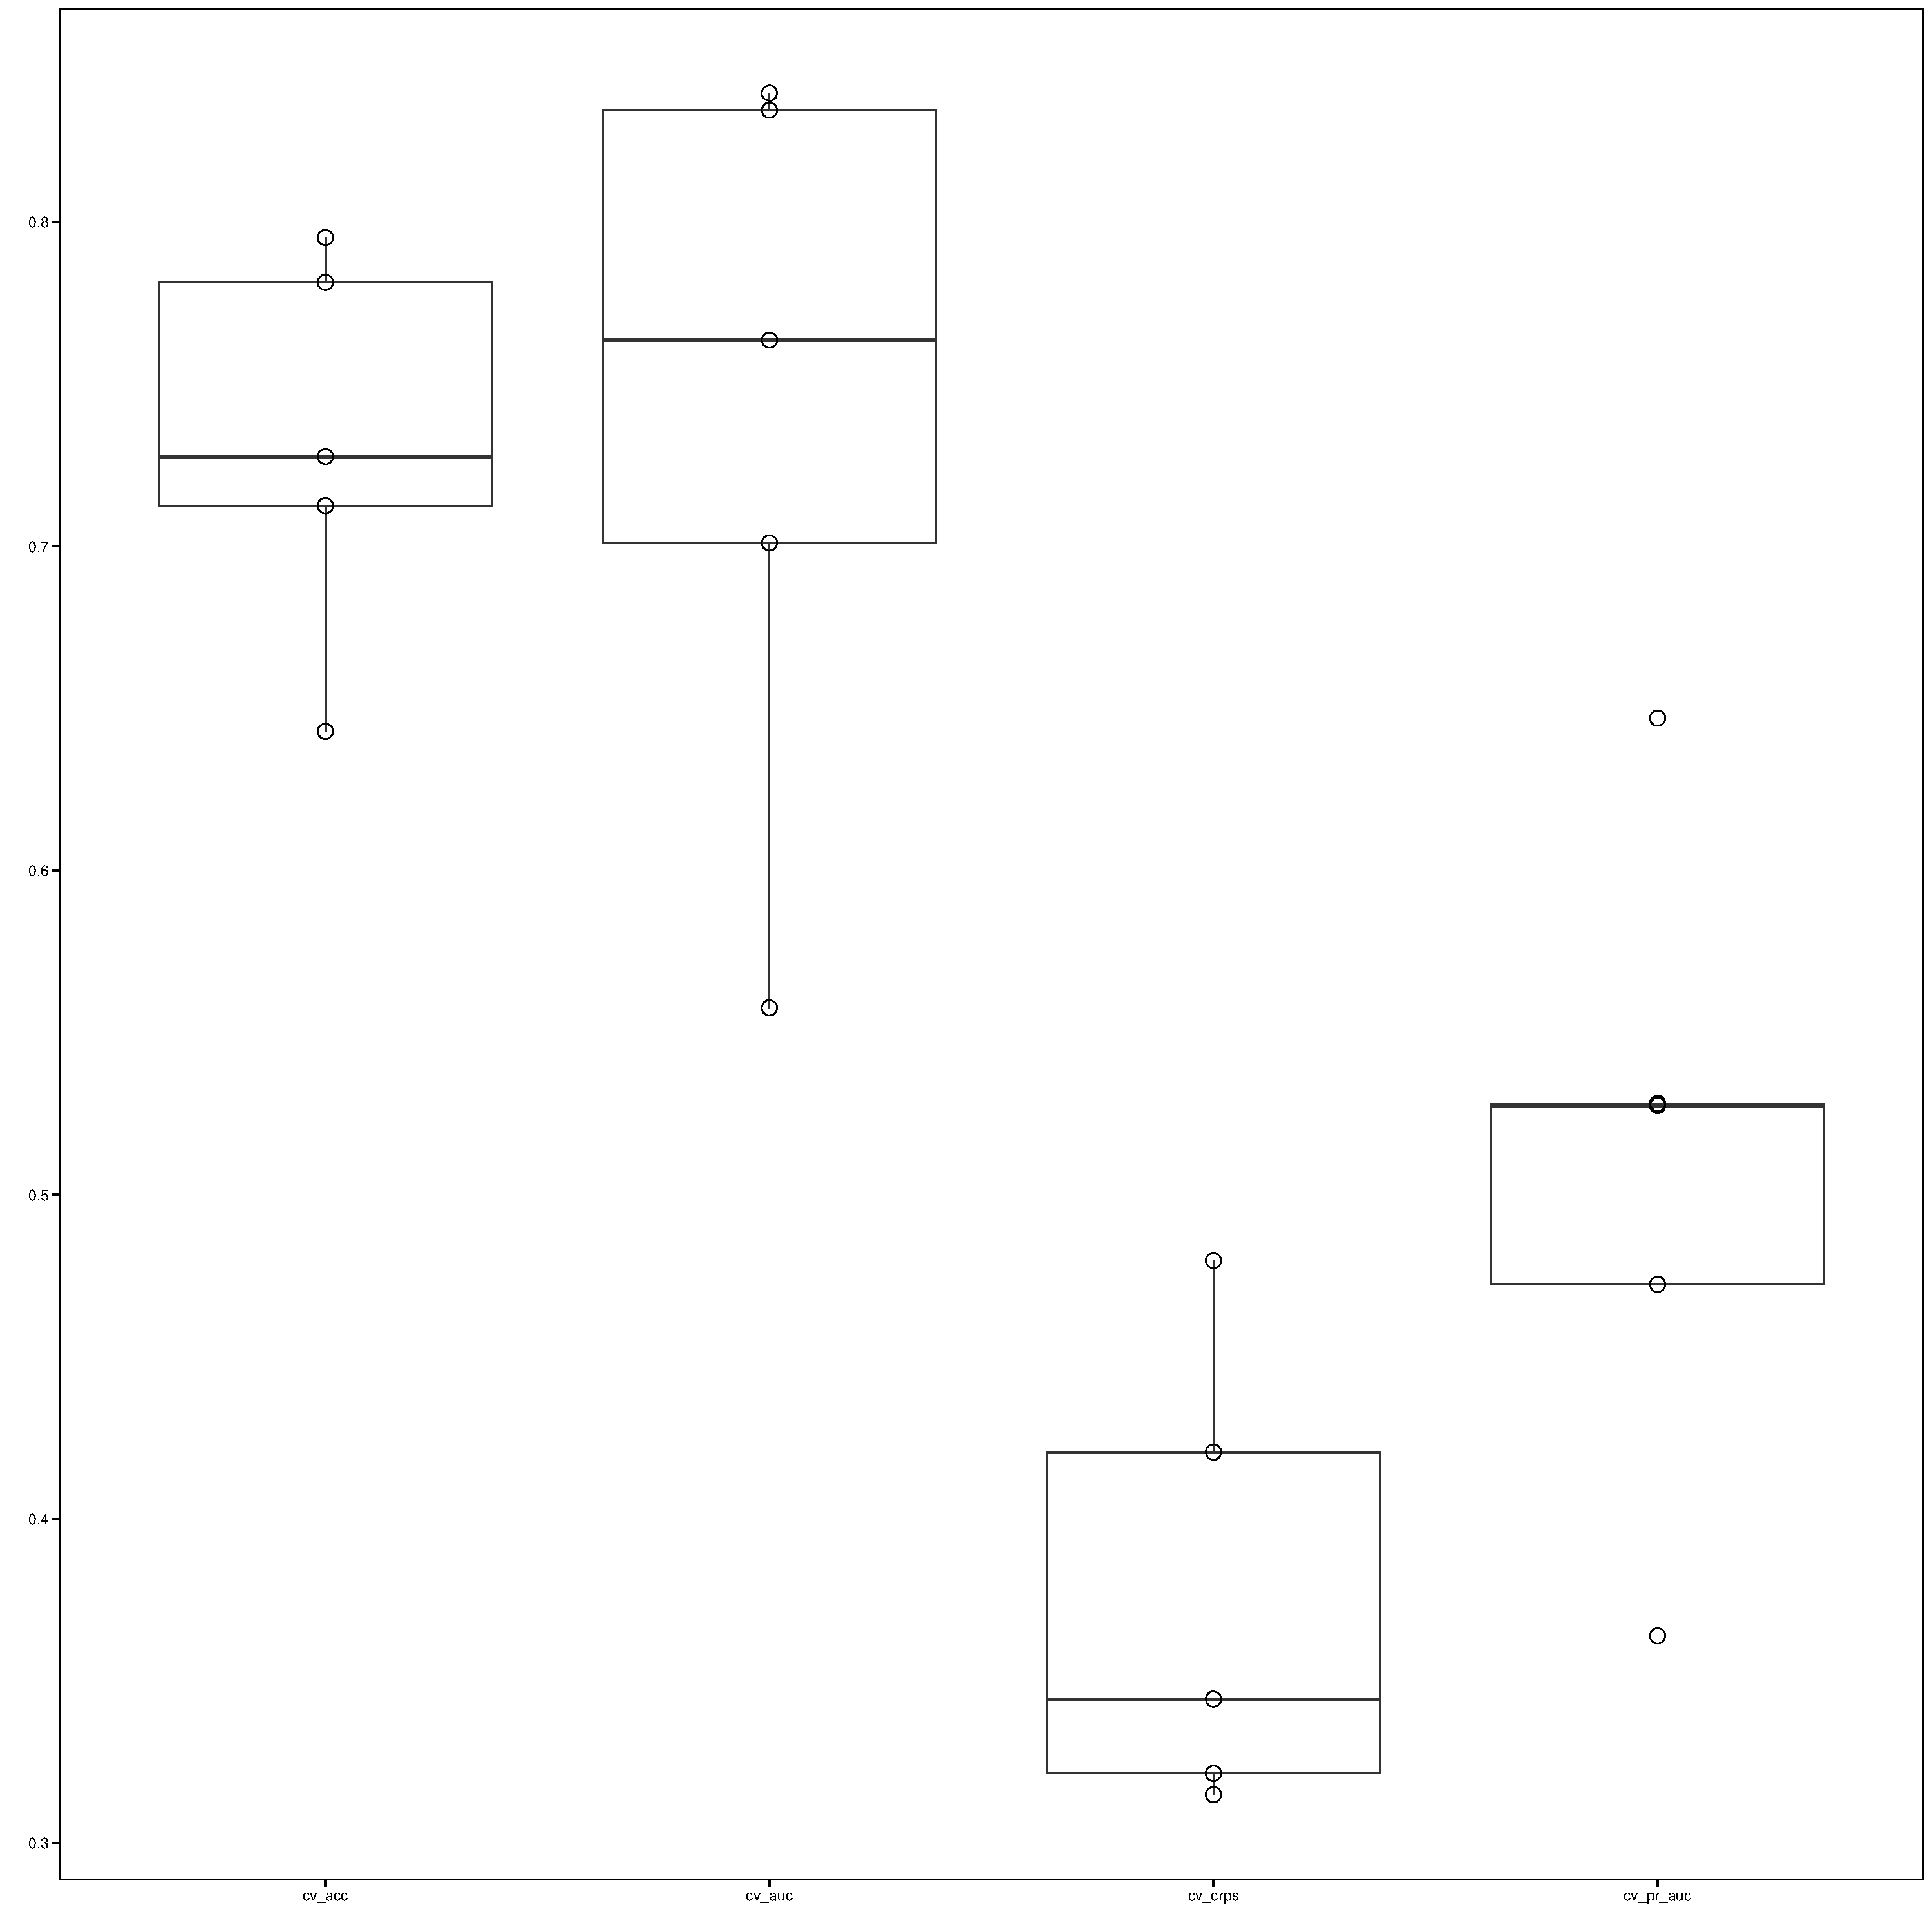
\includegraphics[width=0.75\linewidth]{../figures/rnn_performance_boxplot.pdf}
		\caption{\textbf{Predictive performance of the Teacher RNN across 5-fold LNSO cross-validation.}
			Boxplots display the median and interquartile range (IQR) across validation folds; points represent individual fold scores ($N = 50$ participants, $10$ held-out per fold).
			\textbf{Architecture:} A single-layer Gated Recurrent Unit (GRU, hidden size $H = 4$) evaluated on a $6$-dimensional input vector (boundary targets, lagged rewards, lagged choice, and lagged RT).
			\textbf{Dual Heads:} (1) A policy head predicting choice switching probability using weighted binary cross-entropy. (2) A kinematic head predicting reaction times with a $2$-component shifted Log-Normal mixture, enforcing $\sigma_k > 0$ and non-decision time $\tau_k < \min(\mathrm{RT})$.
			\textbf{Training:} Multi-task loss balanced via learned homoscedastic uncertainty parameters, optimized with Adam ($\eta = 0.002$) over $20$ epochs per fold.
			\textbf{Out-of-Sample Metrics:} Mean $\mathrm{ROC}\text{-}\mathrm{AUC} = 0.795 \pm 0.037$, $\mathrm{PR}\text{-}\mathrm{AUC} = 0.537 \pm 0.078$, $\mathrm{CRPS} = 0.383 \pm 0.079\,\mathrm{s}$ ($M = 200$ Monte Carlo samples), and accuracy $= 0.739 \pm 0.054$.}
		\label{fig:rnn_teacher_lnso}
	\end{figure}
	
	
	
	\printbibliography

\end{document}
